\textbf{Ejemplo 2}\\
Dado el 24\% periodo 3 años vencido, hallar una tasa periódica equivalente para periodo 2 años vencido\\ \\
%\newpage %USAR SOLO SI EL SOLUCIÓN QUEDA SOLO Y ES NECESARIO BAJARLO A LA SIGUIENTE PAGINA
\textbf{Solución.}\\
%La tabla ira centrada
\begin{center}
 \renewcommand{\arraystretch}{1.5}% Margenes de las celdas
 %Creación de la cuadricula de 3 columnas
 \begin{longtable}[H]{|p{0.5\linewidth}|p{0.5\linewidth}|}
  \hline
  \multicolumn{2}{|c|}{\cellcolor[HTML]{FFB183}\textbf{1. Declaración de variables}}                         \\ \hline
  \multicolumn{2}{|c|}{$m=\frac{3}{2}p(2a)v$  $T=8\% $ na$i_1=24\% p(3a)v$  $i_2=?\% p(2a)v$ }              \\ \hline                                         
  \multicolumn{2}{|c|}{\cellcolor[HTML]{FFB183}\textbf{2. Tabla de flujo de caja}}                           \\ \hline
  \multicolumn{2}{|c|}{En este ejercicio, no se realiza la tabla de flujo de caja.}                          \\ \hline
  \multicolumn{2}{|c|}{\cellcolor[HTML]{FFB183}\textbf{3. Fórmulas utilizadas}}                              \\ \hline
  \multicolumn{2}{|l|}{Mediante el uso de Excel:}                                                            \\
  \multicolumn{2}{|l|}{INT.EFECTIVO: Devuelve la tasa de interés anual efectiva}                             \\ \hline
  \multicolumn{2}{|c|}{\cellcolor[HTML]{FFB183}\textbf{4. Desarrollo en Excel}}                              \\ \hline
\multicolumn{2}{|l|}{Se aplicará la función INT.EFECTIVO de la siguiente forma:}                             \\
  \multicolumn{2}{|c|}{ 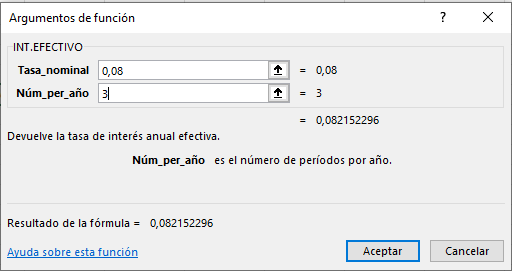
\includegraphics[trim=-5 -5 -5 -5 ,width=1\columnwidth]{2/Ejem2.1.PNG}}              \\
  \multicolumn{2}{|c|}{ 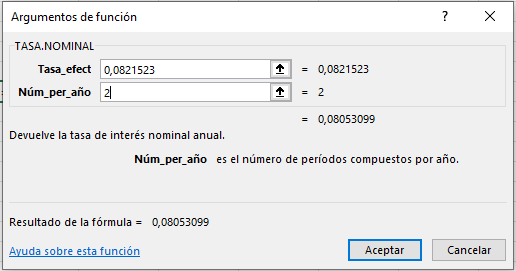
\includegraphics[trim=-5 -5 -5 -5 ,width=1\columnwidth]{2/Ejem2.2.PNG}}
 \\ \hline
  \multicolumn{2}{|c|}{\cellcolor[HTML]{FFB183}\textbf{5. Respuesta}}                                        \\ \hline
  \multicolumn{2}{|c|}{La tasa es del 16,11\% período 2 año vencido}                                        \\ \hline
  \multicolumn{2}{|c|}{\cellcolor[HTML]{FFB183}\textbf{6. Gráfica}}                                          \\ \hline
  \multicolumn{2}{|c|}{No es necesaria la realización de una gráfica para este ejercicio.}                   \\ \hline
 \end{longtable}
 %\newline \newline %USARLO SI CREES QUE ES NECESARIO
\end{center}
